\documentclass[10pt, compress]{beamer}

\usetheme{m}

\usepackage{booktabs}
\usepackage[scale=2]{ccicons}
\usepackage{minted}
\usepackage{tikz}
\usetikzlibrary{calc, arrows}
\usepackage{xstring}
\usepackage{amsmath}
\usepgfplotslibrary{dateplot}
\usemintedstyle{trac}


\usetikzlibrary{shapes,arrows}
\tikzstyle{cloud} = [draw, ellipse, node distance=4cm,    minimum height=2em]
\tikzstyle{cloudgreen} = [draw, ellipse, fill=green!20, node distance=4cm,    minimum height=2em]
\tikzstyle{blockred} = [rectangle, draw, fill=red!20, 
text width=5em, text centered, rounded corners, minimum height=4em, minimum width= 6em]
\tikzstyle{block} = [rectangle, draw, fill=white!20, 
text width=5em, text centered, rounded corners, minimum height=4em,minimum width= 6em]
\tikzstyle{blockgreen} = [rectangle, draw, fill=green!20, 
text width=5em, text centered, rounded corners, minimum height=4em, minimum width= 6em]
\tikzstyle{line} = [draw, -latex']


\renewcommand{\(}{\begin{columns}}
\renewcommand{\)}{\end{columns}}
\newcommand{\<}[1]{\begin{column}{#1}}
	\renewcommand{\>}{\end{column}}
%%%%%%%%%%%%%%%%%%%%%%%%%%%%%%%%%%%%%%%%%%%%%%%%%%
\newcommand*{\NodeSize}{0.5cm}%
\newcommand*{\YShiftBetweenRows}{-1cm}% Subsequent rows are shited down so they don't overlap
\tikzset{DNA Style/.style={minimum size=0.5cm, draw=gray, line width=1pt}}{}

\newlength{\YShift}% 
\newcounter{ColumnCounter}% Prefix for node labels

% Initialize - These are probably not needed, but prefer to set them
\setlength{\YShift}{0cm}% 
\setcounter{ColumnCounter}{0}
\newcommand*{\DNASequence}[2][Mark]{%
	% http://tex.stackexchange.com/questions/12091/tikz-foreach-loop-with-macro-defined-list
	\def\Sequence{#2}
	\foreach [count=\xi] \Label/\Color in \Sequence {%
		\pgfmathsetmacro{\XShift}{\NodeSize*\xi}%
		\IfStrEq{\Color}{}{\def\Color{white}}{}
		\edef\NodeName{#1-\arabic{ColumnCounter}}
		\node [DNA Style, fill=\Color, xshift=\XShift] (\NodeName) {\Label};
		\stepcounter{ColumnCounter}
	} 
}%
\newcommand*{\ThreeDNASequences}[4][Mark]{% #1 = tikzmark prefix
	\setcounter{ColumnCounter}{0}% reset column counter
	\begin{scope}[yshift=\YShift]
		\DNASequence[#1]{#2} 
		\pgfmathsetmacro{\Shift}{6cm}% Should compute this based on num of items in #1
		\begin{scope}[xshift=\Shift]
			\DNASequence[#1]{#3} 
		\end{scope}
		\pgfmathsetmacro{\Shift}{8cm}% Should compute this based on num of items in #2  
		\begin{scope}[xshift=\Shift]
			\DNASequence[#1]{#4} 
		\end{scope}
	\end{scope}
	\pgfmathsetlength{\YShift}{\YShift\YShiftBetweenRows}%
}

\title{Parallel single-cell sequencing links transcriptional and epigenetic heterogeneity
	}
\subtitle{Angermueller et al., Nature Methods, January 11, 2016. doi:10.1038/nmeth.3728.}


\vspace*{20pt}
\author[skc]{Saket Choudhary}
%\institute{\inst{1} University of Southern California}

\date{%\vspace*{50pt}
\today \\
BISC 542}

\begin{document}

\maketitle


\begin{frame}[fragile]
\begin{center}
\Large scM\&T-seq: Parallel single-cell genome-wide methylation \& transcriptome seq\\ 
$\implies$ Coupled/Uncoupled?
\end{center}
\end{frame}

\begin{frame}[fragile]
%	\frametitle{Protocol}
	\centering \Large Protocol
	\vspace*{-7pt}
	\begin{center}
	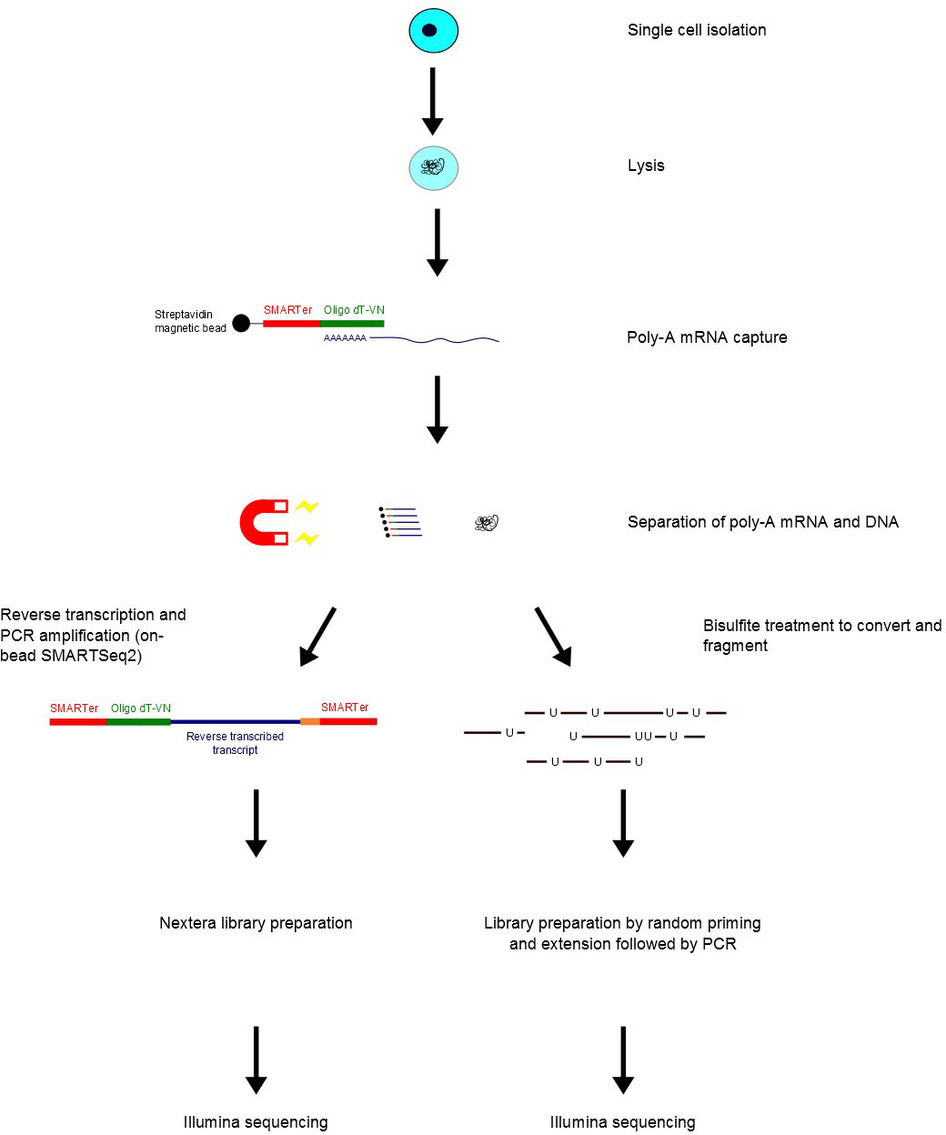
\includegraphics[width=\linewidth,height=\textheight,keepaspectratio]{images/protocol}
\end{center}
\end{frame}

\begin{frame}[fragile]
	\begin{center} \Huge Data:\end{center}
	\begin{center}
\Large 	76 individual serum ESC + 16 ESCc in `2i'[induces hypomethylation]
\end{center}
\end{frame}

\begin{frame}[fragile]
	\begin{center} \large Variation in methylation levels are explained by cell type \end{center}
	\vspace*{-20pt}
	\begin{center}
		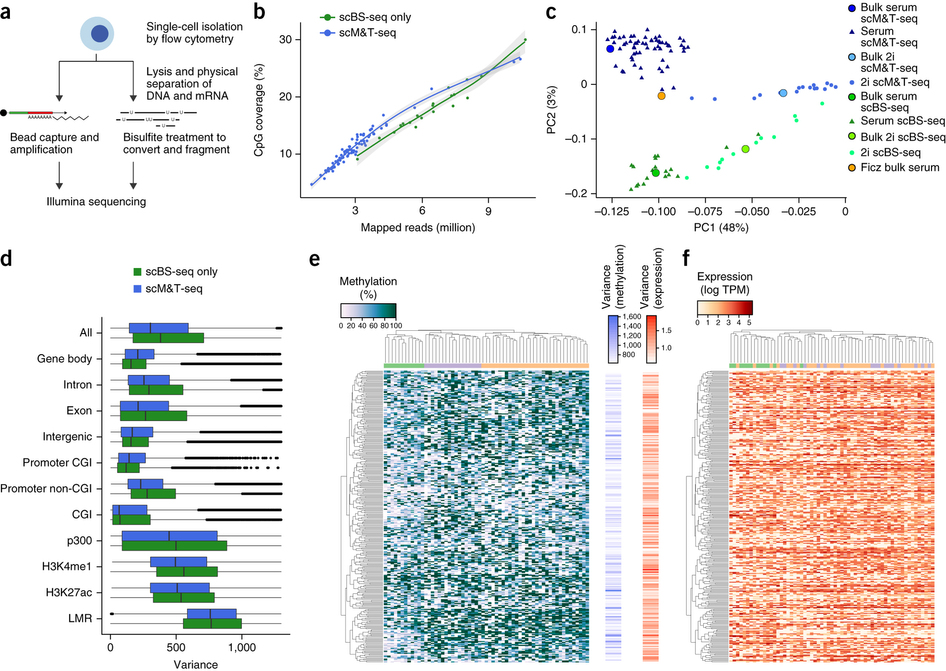
\includegraphics[width=\linewidth,height=\textheight,keepaspectratio]{images/result1}
		\end{center}
\end{frame}


\begin{frame}[fragile]
\centering \large Methylation PCs partially recapitulate expression %structure 
	\vspace*{-10pt}
	\begin{center}
		
		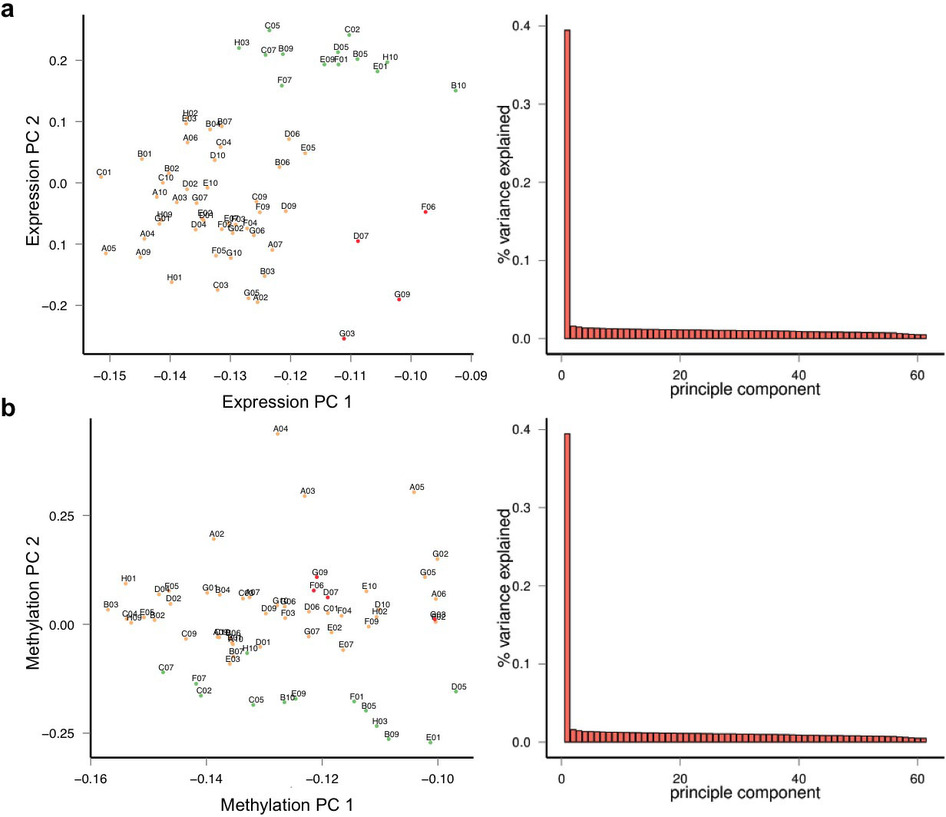
\includegraphics[width=\linewidth,height=\textheight,keepaspectratio]{images/pca1}
		%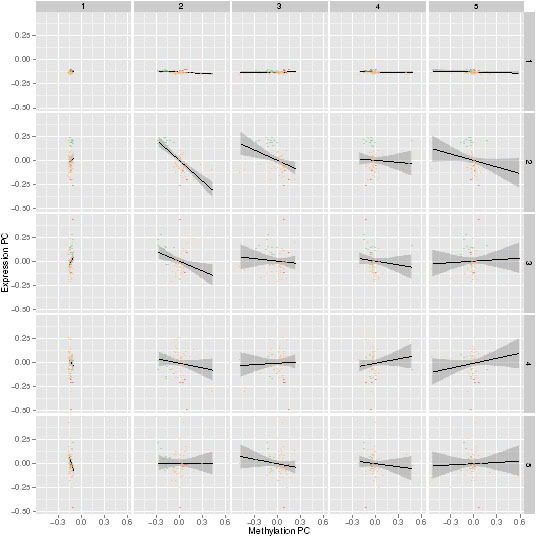
\includegraphics[width=0.5\linewidth,height=\textheight,keepaspectratio]{images/pca2}
	\end{center}
\end{frame}

\begin{frame}[fragile]
		\centering \large Methylation PCs correlate with Expression PCs
	\vspace*{-12pt}
	\begin{center}
		
		%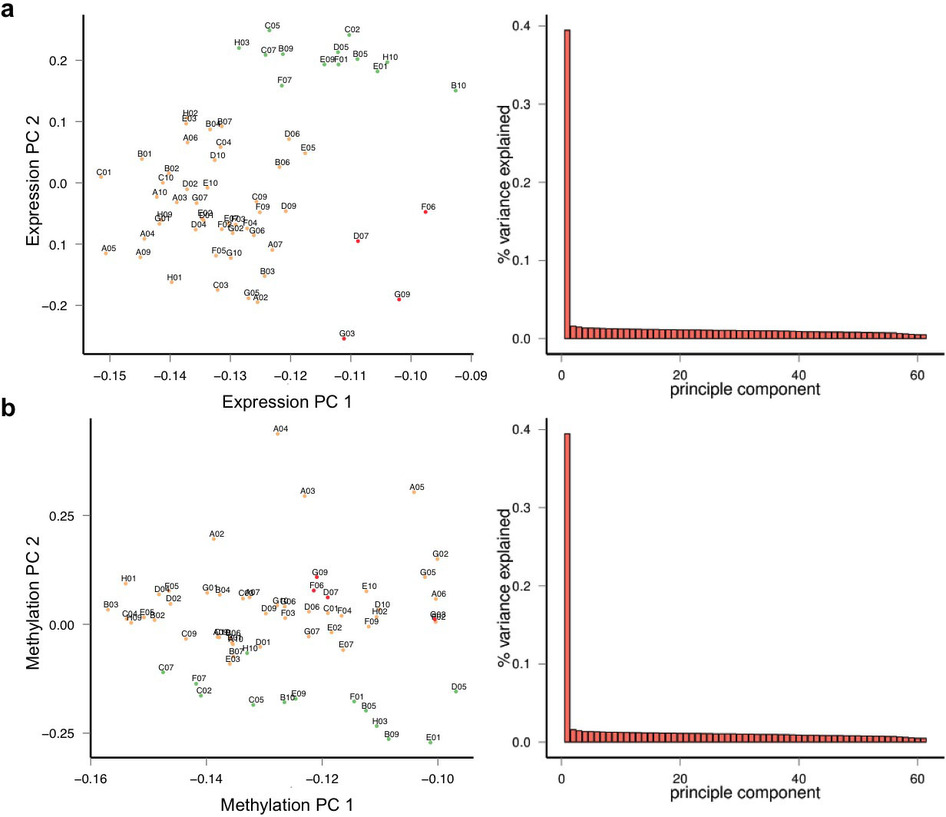
\includegraphics[width=0.5\linewidth,height=\textheight,keepaspectratio]{images/pca1}
		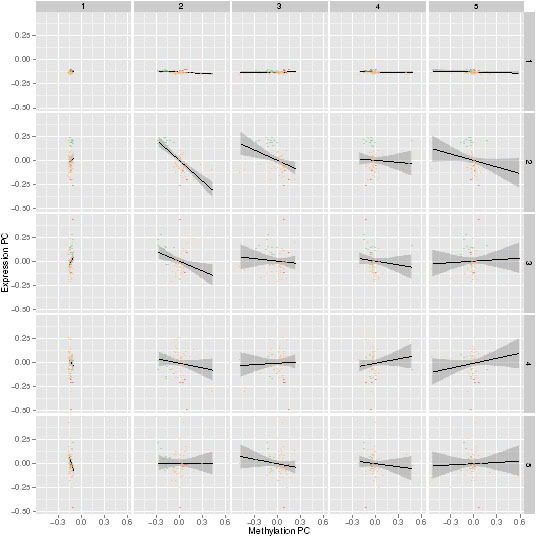
\includegraphics[width=\linewidth,height=\textheight,keepaspectratio]{images/pca2}
	\end{center}
\end{frame}
	
\begin{frame}[fragile]
	\begin{center}\large{Global methylome and transcriptome profiles are complementary}\end{center}
	\vspace*{-10pt}
	\begin{center}
		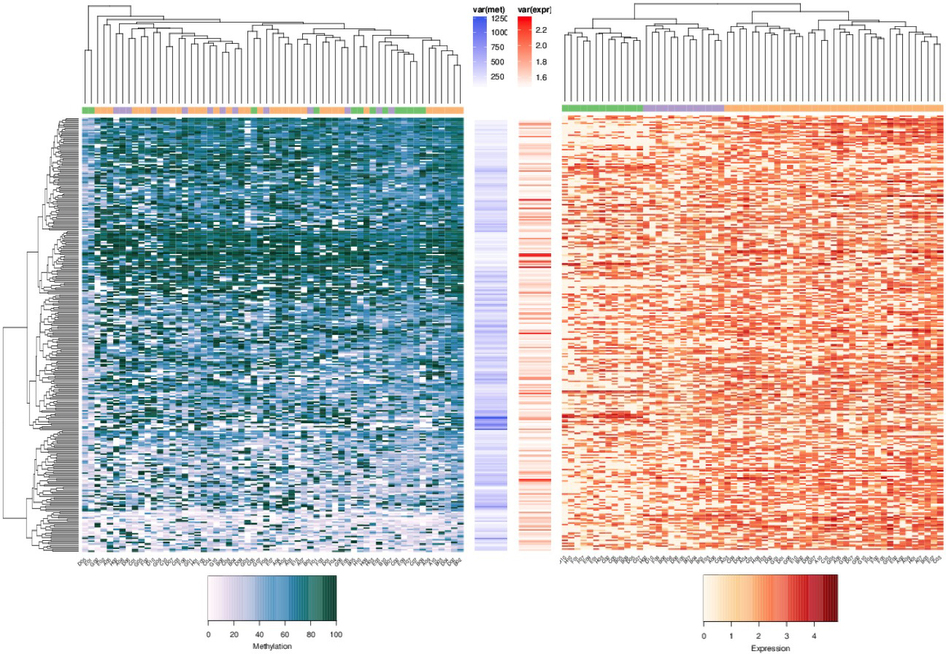
\includegraphics[width=\linewidth,height=\textheight,keepaspectratio]{images/clustering}
	\end{center}
\end{frame}

\begin{frame}[fragile]
	\begin{center}
	\huge  
	Association between expression levels and methylation : BOTH negative and positive $\implies$ Interactions are Complex!
	\end{center}
\end{frame}

\begin{frame}
	\begin{center} \large Correlation coefficients in alternative genomic context: \end{center}
	\vspace*{-10pt}
	\begin{center}
		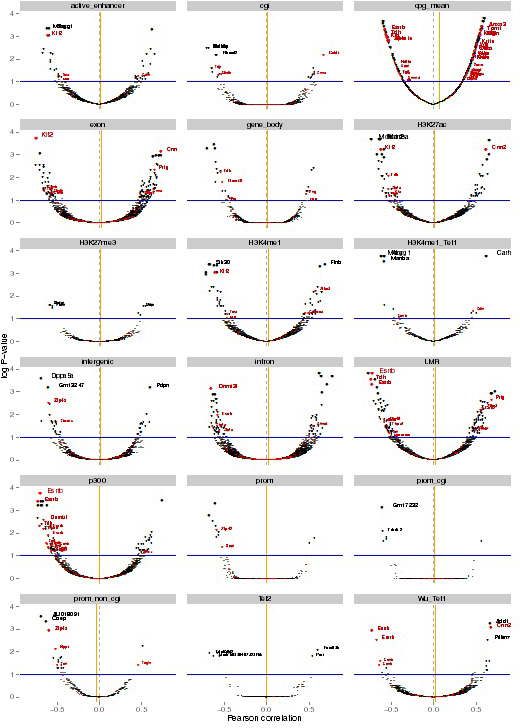
\includegraphics[width=\linewidth,height=\textheight,keepaspectratio]{images/corr1}
	\end{center}
\end{frame}

\begin{frame}
	
		\begin{center} \Large Validates with bulk RNA-seq and BS-seq[Oranges]	\end{center}
	\begin{center}
		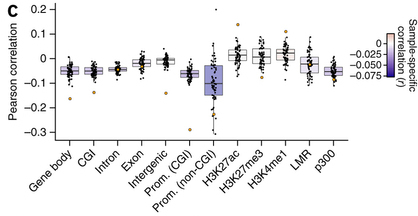
\includegraphics[width=\linewidth,height=\textheight,keepaspectratio]{images/corr2}
	\end{center}
\end{frame}

\begin{frame}[fragile]
	\begin{center} \Huge Insights \end{center}
	
 	\centering \Large Transcriptome and Methylome can be uncoupled
	
\end{frame}

\begin{frame}[fragile]
	\begin{center}	 \Huge Insights \end{center}
\Large Association with transcription: \begin{itemize}
	\item v/s methylation at non-CpG island promoters : negative (known)
	\item v/s methylation at distal regulatory elements : both
\end{itemize}
\end{frame}



\begin{frame}[fragile]
	\centering \Huge Summary
\Large \begin{itemize}
		\item Parallel methylome \& transcriptome profiling: feasbile
		\item Associations can be quantified at single-cell level
		\item Fluctuating pluripotency in serum ESC $\cong$ Epigenetic heterogenity
	\end{itemize}
\end{frame}




\begin{frame}[fragile]
	\centering \Large {References}
	\footnotesize
	\begin{itemize}
		\item Seisenberger, Stefanie, et al. "The dynamics of genome-wide DNA methylation reprogramming in mouse primordial germ cells." Molecular cell 48.6 (2012): 849-862.
		\item Han, Han, et al. "DNA methylation directly silences genes with non-CpG island promoters and establishes a nucleosome occupied promoter." Human molecular genetics (2011): ddr356.
		\item Ficz, Gabriella, et al. "Dynamic regulation of 5-hydroxymethylcytosine in mouse ES cells and during differentiation." Nature 473.7347 (2011): 398-402. 
		\item Macaulay, Iain C., et al. "G\&T-seq: parallel sequencing of single-cell genomes and transcriptomes." Nature methods 12.6 (2015): 519-522.
		\item Smallwood, Sébastien A., et al. "Single-cell genome-wide bisulfite sequencing for assessing epigenetic heterogeneity." Nature methods 11.8 (2014): 817-820.
		\item Yang, Xiaojing, et al. "Gene body methylation can alter gene expression and is a therapeutic target in cancer." Cancer cell 26.4 (2014): 577-590.
		\item Bogdanović, Ozren, et al. "Temporal uncoupling of the DNA methylome and transcriptional repression during embryogenesis." Genome research 21.8 (2011): 1313-1327.
	\end{itemize}
\end{frame}

\end{document}
